\documentclass[aspectratio=169, table]{beamer}

%\usepackage[beamertheme=./praditatheme]{Pradita}
\usepackage[utf8]{inputenc}
\usepackage{xcolor} % for color
\usepackage{colortbl} % for table color
\usepackage{listings}

% Define Java language style for listings
\lstdefinestyle{JavaStyle}{
language=Java,
basicstyle=\ttfamily\tiny,
keywordstyle=\color{blue},
commentstyle=\color{gray},
stringstyle=\color{red},
breaklines=true,
showstringspaces=false,
tabsize=2,
captionpos=b,
numbers=left,
numberstyle=\tiny\color{gray},
frame=lines,
backgroundcolor=\color{lightgray!10},
comment=[l]{//},
morecomment=[s]{/*}{*/},
commentstyle=\color{gray}\ttfamily,
string=[s]{'}{'},
morestring=[s]{"}{"},
%	stringstyle=\color{teal}\ttfamily,
%	showstringspaces=false
}

\lstdefinestyle{sql}{
language=sql,
keywords={use, insert, into, values, select, from,
update, set, delete, create, where, join, left, right, inner, order, by, primary, key},
ndkeywords={max, min, varchar, int},
ndkeywordstyle=\color{purple}\bfseries,
basicstyle=\ttfamily\scriptsize,
keywordstyle=\color{blue},
commentstyle=\color{gray},
stringstyle=\color{red},
breaklines=true,
showstringspaces=false,
tabsize=2,
captionpos=b,
numbers=left,
numberstyle=\tiny\color{gray},
frame=lines,
backgroundcolor=\color{lightgray!10},
comment=[l]{\#},
morecomment=[s]{/*}{*/},
commentstyle=\color{gray}\ttfamily,
string=[s]{'}{'},
morestring=[s]{"}{"},
%	stringstyle=\color{teal}\ttfamily,
%	showstringspaces=false
}

\lstdefinelanguage{bash} {
keywords={},
basicstyle=\ttfamily\scriptsize,
keywordstyle=\color{blue}\bfseries,
ndkeywords={iex},
ndkeywordstyle=\color{purple}\bfseries,
sensitive=true,
commentstyle=\color{gray},
stringstyle=\color{red},
numbers=left,
numberstyle=\tiny\color{gray},
breaklines=true,
frame=lines,
backgroundcolor=\color{lightgray!10},
tabsize=2,
comment=[l]{\#},
morecomment=[s]{/*}{*/},
commentstyle=\color{gray}\ttfamily,
stringstyle=\color{purple}\ttfamily,
showstringspaces=false
}

\lstdefinestyle{XmlStyle} {
language=xml,
keywords={xmlns,version,type,import},
basicstyle=\ttfamily\scriptsize,
keywordstyle=\color{blue}\bfseries,
ndkeywords={import},
ndkeywordstyle=\color{purple}\bfseries,
sensitive=true,
commentstyle=\color{gray},
stringstyle=\color{red},
numbers=left,
numberstyle=\tiny\color{gray},
breaklines=true,
frame=lines,
backgroundcolor=\color{lightgray!10},
tabsize=2,
showstringspaces=false,
comment=[l]{\#},
commentstyle=\color{gray}\ttfamily,
stringstyle=\color{purple}\ttfamily,
morecomment=[s]{<!--}{-->}
}

\lstdefinelanguage{css}{
basicstyle=\ttfamily\footnotesize,
keywordstyle=\color{blue},
commentstyle=\color{gray},
stringstyle=\color{red},
breaklines=true,
showstringspaces=false,
tabsize=2,
captionpos=b,
numbers=left,
numberstyle=\tiny\color{gray},
frame=lines,
backgroundcolor=\color{lightgray!10},
comment=[l]{//},
morecomment=[s]{/*}{*/},
commentstyle=\color{gray}\ttfamily,
string=[s]{'}{'},
morestring=[s]{"}{"},
%	stringstyle=\color{teal}\ttfamily,
%	showstringspaces=false
}

\usetheme{Pradita}

\subtitle{IF220303 - Object-oriented Programming}

\title{\Huge Advanced JavaFX\\\vspace{20pt}}
\date[Serial]{\scriptsize {PRU/SPMI/FR-BM-18/0222}}
\author[Pradita]{\small {\textbf{Alfa Yohannis}}}

\begin{document}

\frame{\titlepage}

\begin{frame}[fragile]
\frametitle{Contents}
\vspace{10pt}
\begin{columns}[t]
	\column{0.5\textwidth}
	\tableofcontents[sections={1-5}]
	
	\column{0.5\textwidth}
	\tableofcontents[sections={6-10}]
\end{columns}
\end{frame}

\section{MVC}
\begin{frame}{Model-View-Controller (MVC) in JavaFX}
\vspace{20pt}
\textbf{Model-View-Controller (MVC)} is an architectural pattern that separates business logic, presentation, and user interaction into three main components:
\begin{itemize}
	\item \textbf{Model} – Responsible for managing data and business logic.
	\item \textbf{View} – Displays information to the user through a graphical interface.
	\item \textbf{Controller} – Connects user interactions with the Model and updates the View accordingly.
\end{itemize}
\vspace{10pt}
\textbf{Advantages of MVC in JavaFX:}
\begin{itemize}
	\item Clear separation between logic and presentation improves modularity.
	\item Facilitates maintenance and further application development.
	\item Enables more effective unit testing for each component.
\end{itemize}
\end{frame}

\begin{frame}{Model-View-Controller Architecture Structure}
\vspace{20pt}
\begin{figure}[ht]
	\centering
	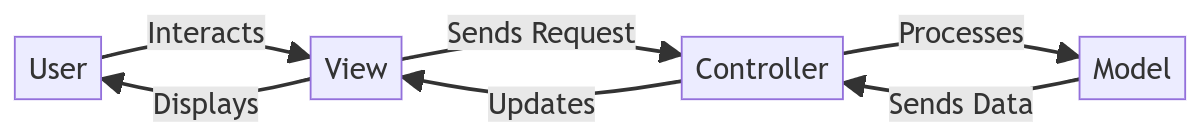
\includegraphics[width=0.9\textwidth]{../../figures/mvc-modern.png}
	\label{fig:mvc_architecture}
\end{figure}
\vspace{10pt}
The diagram above illustrates the data flow in the MVC architecture.
\begin{itemize}
	\item Users interact with the \textbf{View} through UI elements.
	\item \textbf{Controller} handles user actions and forwards them to the Model.
	\item \textbf{Model} processes the data and returns it to the Controller.
	\item \textbf{Controller} updates the View with the latest data from the Model.
\end{itemize}
\end{frame}

\section{Prerequisites}
\begin{frame}{Java and MySQL Prerequisites}
\vspace{20pt}
Before starting JavaFX application development, ensure that the following software is installed:
\begin{itemize}
	\item Java Development Kit (JDK) version 11 or newer.
	\item MySQL as the database for application data storage.
	\item MySQL JDBC Driver to allow Java to communicate with the database.
	\item Gradle as a build tool for managing dependencies and automating the project build process.
\end{itemize}
\end{frame}
\section{Gradle}
\subsection{Gradle Initialization}
\begin{frame}[fragile]{Creating and Initializing a Java Project with Gradle}
\vspace{20pt}
To start a new Java project with Gradle, first create a project directory and navigate into it:

\begin{lstlisting}[language=bash]
	mkdir my-java-project
	cd my-java-project
\end{lstlisting}

Then, initialize the project using Gradle:

\begin{lstlisting}[language=bash]
	gradle init --type java-application
\end{lstlisting}

Gradle will prompt for several configuration options, as shown in the next section.
\end{frame}

\begin{frame}[fragile]{Gradle Initialization Configuration}
\vspace{30pt}
Gradle requires user input during initialization:

\begin{lstlisting}[language=bash]
	Enter target Java version (min: 7, default: 21): 21
	Project name (default: dummy): dummy
	
	Select application structure:
	1: Single application project
	2: Application and library project
	Enter selection (default: Single application project) [1..2] 1
	
	Select build script DSL:
	1: Kotlin
	2: Groovy
	Enter selection (default: Kotlin) [1..2] 2
	
	Select test framework:
	1: JUnit 4
	2: TestNG
	3: Spock
	4: JUnit Jupiter
	Enter selection (default: JUnit Jupiter) [1..4] 4
\end{lstlisting}
\end{frame}

\begin{frame}[fragile]{Finalizing the Gradle Initialization}
\vspace{20pt}
Complete the Gradle setup by confirming the API behavior:

\begin{lstlisting}[language=bash]
	Generate build using new APIs and behavior (some features may change in the next minor release)? (default: no) [yes, no] no
	
	> Task :init
	Learn more about Gradle by exploring our Samples at 
	https://docs.gradle.org/8.13/samples/sample_building_java_applications.html
	
	BUILD SUCCESSFUL in 32s
	1 actionable task: 1 executed
\end{lstlisting}

The Java project is now initialized and ready for development.
\end{frame}

\subsection{Gradle Project}
\begin{frame}[fragile]{JavaFX Project Structure (Part 1)}
\vspace{20pt}
\begin{lstlisting}[language=bash]
	my-javafx-project/
	|-- app/
	|   |-- build.gradle
	|   |-- src/
	|   |   |-- main/
	|   |   |   |-- java/
	|   |   |   |   |-- org/example/controllers/
	|   |   |   |   |   |-- ItemController.java
	|   |   |   |   |   |-- MainController.java
	|   |   |   |   |   |-- SalesOrderController.java
	|   |   |   |   |   |-- SelectFormController.java
	|   |   |   |   |-- org/example/helpers/
	|   |   |   |   |   |-- IForm.java
	|   |   |   |   |-- org/example/models/
	|   |   |   |   |   |-- Item.java
	|   |   |   |   |   |-- Order.java
	|   |   |   |   |   |-- OrderDetail.java
	|   |   |   |   |   |-- OrderDetailPK.java
\end{lstlisting}
\end{frame}

\begin{frame}[fragile]{JavaFX Project Structure (Part 2)}
\vspace{20pt}
\begin{lstlisting}[language=bash]
	|   |   |   |-- resources/
	|   |   |   |   |-- hibernate.cfg.xml
	|   |   |   |   |-- Item.fxml
	|   |   |   |   |-- Main.fxml
	|   |   |   |   |-- SalesOrder.fxml
	|   |   |   |   |-- SelectForm.fxml
	|   |   |   |   |-- test.rptdesign
	|-- settings.gradle
	|-- gradle.properties
	|-- gradlew
	|-- gradlew.bat
\end{lstlisting}
\end{frame}

\subsection{Gradle Configuration}
\begin{frame}[fragile]{Gradle Build Configuration (Part 1)}
\vspace{20pt}
\begin{lstlisting}[style=JavaStyle]
	plugins {
		id 'application'
		id 'org.openjfx.javafxplugin' version '0.1.0'
	}
	
	repositories {
		mavenCentral()
	}
	
	dependencies {
		implementation 'mysql:mysql-connector-java:8.0.33'
		implementation 'org.hibernate:hibernate-core:6.2.12.Final'
		implementation 'jakarta.persistence:jakarta.persistence-api:3.1.0'
		implementation "org.openjfx:javafx-controls:20.0.1"
		implementation "org.openjfx:javafx-fxml:20.0.1"
		implementation 'com.innoventsolutions.birt.runtime:org.eclipse.birt.runtime_4.8.0-20180626:4.8.0'
	\end{lstlisting}
\end{frame}

\begin{frame}[fragile]{Gradle Build Configuration (Part 2)}
	\vspace{20pt}
	\begin{lstlisting}[style=JavaStyle]
		testImplementation libs.junit.jupiter
		testRuntimeOnly 'org.junit.platform:junit-platform-launcher'
		implementation libs.guava
	}
	
	java {
		toolchain {
			languageVersion = JavaLanguageVersion.of(21)
		}
	}
	
	application {
		mainClass = 'org.example.Main'
	}
	
	tasks.named('test') {
		useJUnitPlatform()
	}
	
	javafx {
		version = "21.0.1"
		modules = [ 'javafx.controls', 'javafx.fxml' ]
	}
\end{lstlisting}
\end{frame}

\section{Hibernate Configuration}
\begin{frame}[fragile]{Hibernate Configuration (Part 1)}
\vspace{20pt}
\begin{lstlisting}[style=XmlStyle]
	<?xml version="1.0" encoding="utf-8"?>
	<!DOCTYPE hibernate-configuration PUBLIC 
	"-//Hibernate/Hibernate Configuration DTD 3.0//EN"
	"http://www.hibernate.org/dtd/hibernate-configuration-3.0.dtd">
	<hibernate-configuration>
	<session-factory>
	<!-- Database Configuration -->
	<property name="hibernate.connection.driver_class">
	com.mysql.cj.jdbc.Driver
	</property>
	<property name="hibernate.connection.url">
	jdbc:mysql://localhost:3306/pradita?useSSL=false&amp;serverTimezone=UTC
	</property>
	<property name="hibernate.connection.username">alfa</property>
	<property name="hibernate.connection.password">1234</property>
\end{lstlisting}
\end{frame}

\begin{frame}[fragile]{Hibernate Configuration (Part 2)}
\vspace{20pt}
\begin{lstlisting}[style=XmlStyle]
	<!-- Hibernate Settings -->
	<property name="hibernate.dialect">org.hibernate.dialect.MySQLDialect</property>
	<property name="hibernate.show_sql">true</property>
	<property name="hibernate.format_sql">true</property>
	<property name="hibernate.hbm2ddl.auto">update</property>
	
	<!-- Entity Mappings -->
	<mapping class="org.example.models.Order"/>
	<mapping class="org.example.models.OrderDetail"/>
	<mapping class="org.example.models.Item"/>
	</session-factory>
	</hibernate-configuration>
\end{lstlisting}
\end{frame}

\section{Models}
\subsection{Item.java}
\begin{frame}[fragile]{Item.java (Part 1)}
\vspace{20pt}
\begin{lstlisting}[style=JavaStyle]
	package org.example.models;
	
	import jakarta.persistence.Column;
	import jakarta.persistence.Entity;
	import jakarta.persistence.Id;
	import jakarta.persistence.Table;
	
	@Entity
	@Table(name = "item")
	public class Item {
		@Id
		@Column(name = "code", length = 5, nullable = false)
		private String code;
		
		@Column(name = "name", length = 50)
		private String name;
		
		@Column(name = "price", nullable = false)
		private Double price;
		
		@Column(name = "quantity", nullable = false)
		private Double quantity;
	\end{lstlisting}
\end{frame}

\begin{frame}[fragile]{Item.java (Part 2)}
	\vspace{20pt}
	\begin{lstlisting}[style=JavaStyle]
		// Getters and setters
		public String getCode() { return code; }
		public void setCode(String code) { this.code = code; }
		
		public String getName() { return name; }
		public void setName(String name) { this.name = name; }
		
		public Double getPrice() { return price; }
		public void setPrice(Double price) { this.price = price; }
		
		public Double getQuantity() { return quantity; }
		public void setQuantity(Double quantity) { this.quantity = quantity; }
	}
\end{lstlisting}
\end{frame}

\subsection{Order.java}
\begin{frame}[fragile]{Order.java (Part 1)}
\vspace{20pt}
\begin{lstlisting}[style=JavaStyle]
	package org.example.models;
	
	import java.time.LocalDateTime;
	import java.util.List;
	
	import jakarta.persistence.CascadeType;
	import jakarta.persistence.Column;
	import jakarta.persistence.Entity;
	import jakarta.persistence.Id;
	import jakarta.persistence.OneToMany;
	import jakarta.persistence.Table;
	
	@Entity
	@Table(name = "order")
	public class Order {
		@Id
		@Column(name = "code", length = 5, nullable = false)
		private String code;
		
		@Column(name = "note", columnDefinition = "TEXT")
		private String note;
		
		@Column(name = "date", columnDefinition = 
		"DATETIME DEFAULT CURRENT_TIMESTAMP")
		private LocalDateTime date;
	\end{lstlisting}
\end{frame}

\begin{frame}[fragile]{Order.java (Part 2)}
	\vspace{20pt}
	\begin{lstlisting}[style=JavaStyle]
		@OneToMany(mappedBy = "order", cascade = CascadeType.ALL, 
		orphanRemoval = true)
		private List<OrderDetail> orderDetails;
		
		// Getters and setters
		public String getCode() { return code; }
		public void setCode(String code) { this.code = code; }
		
		public String getNote() { return note; }
		public void setNote(String note) { this.note = note; }
		
		public LocalDateTime getDate() { return date; }
		public void setDate(LocalDateTime date) { this.date = date; }
		
		public List<OrderDetail> getOrderDetails() { return orderDetails; }
		public void setOrderDetails(List<OrderDetail> orderDetails) { 
			this.orderDetails = orderDetails; }
	}
\end{lstlisting}
\end{frame}

\subsection{OrderDetail.java}
\begin{frame}[fragile]{OrderDetail.java (Part 1)}
\vspace{20pt}
\begin{lstlisting}[style=JavaStyle]
	package org.example.models;
	
	import jakarta.persistence.Column;
	import jakarta.persistence.EmbeddedId;
	import jakarta.persistence.Entity;
	import jakarta.persistence.JoinColumn;
	import jakarta.persistence.ManyToOne;
	import jakarta.persistence.MapsId;
	import jakarta.persistence.Table;
	
	@Entity
	@Table(name = "order_detail")
	public class OrderDetail {
		@EmbeddedId
		private OrderDetailPK id;
		
		@ManyToOne
		@MapsId("orderCode")
		@JoinColumn(name = "code", nullable = false)
		private Order order;
		
		@Column(name = "itemcode", length = 5, nullable = false)
		private String itemCode;
	\end{lstlisting}
\end{frame}

\begin{frame}[fragile]{OrderDetail.java (Part 2)}
	\vspace{20pt}
	\begin{lstlisting}[style=JavaStyle]
		@Column(name = "name", length = 50)
		private String name;
		
		@Column(name = "price", nullable = false)
		private Double price;
		
		@Column(name = "quantity", nullable = false)
		private Double quantity;
		
		public OrderDetail() {}
		
		public OrderDetail(OrderDetailPK id, Order order,
		String itemCode, String name, double price,
		double quantity) {
			this.id = id;
			this.order = order;
			this.itemCode = itemCode;
			this.name = name;
			this.price = price;
			this.quantity = quantity;
		}
	\end{lstlisting}
\end{frame}

\begin{frame}[fragile]{OrderDetail.java (Part 3)}
	\vspace{20pt}
	\begin{lstlisting}[style=JavaStyle]
		// Getters and setters
		public OrderDetailPK getId() { return id; }
		public void setId(OrderDetailPK id) { this.id = id; }
		
		public Order getOrder() { return order; }
		public void setOrder(Order order) { this.order = order; }
		
		public String getItemCode() { return itemCode; }
		public void setItemCode(String itemCode) { this.itemCode = itemCode; }
		
		public String getName() { return name; }
		public void setName(String name) { this.name = name; }
		
		public Double getPrice() { return price; }
		public void setPrice(Double price) { this.price = price; }
		
		public Double getQuantity() { return quantity; }
		public void setQuantity(Double quantity) { this.quantity = quantity; }
	}
\end{lstlisting}
\end{frame}

\subsection{OrderDetailPK.java}
\begin{frame}[fragile]{OrderDetailPK.java (Part 1)}
\vspace{20pt}
\begin{lstlisting}[style=JavaStyle]
package org.example.models;

import java.util.Objects;
import jakarta.persistence.Column;
import jakarta.persistence.Embeddable;

@Embeddable
public class OrderDetailPK implements java.io.Serializable {
	@Column(name = "code", length = 5, nullable = false)
	private String orderCode;
	
	@Column(name = "line", nullable = false)
	private Integer line;
	
	public OrderDetailPK() {}
	
	public OrderDetailPK(String newCode, int line) {
		this.orderCode = newCode;
		this.line = line;
	}
	
	// Getters and setters
	public String getOrderCode() { return orderCode; }
	public void setOrderCode(String orderCode) { this.orderCode = orderCode; }
	
	public Integer getLine() { return line; }
	public void setLine(Integer line) { this.line = line; }
\end{lstlisting}
\end{frame}

\begin{frame}[fragile]{OrderDetailPK.java (Part 2)}
\vspace{20pt}
\begin{lstlisting}[style=JavaStyle]
	@Override
	public boolean equals(Object o) {
		if (this == o) return true;
		if (o == null || getClass() != o.getClass()) return false;
		OrderDetailPK that = (OrderDetailPK) o;
		return Objects.equals(orderCode, that.orderCode) && 
		Objects.equals(line, that.line);
	}
	
	@Override
	public int hashCode() {
		return Objects.hash(orderCode, line);
	}
}
\end{lstlisting}
\end{frame}


\section{Controllers}
\subsection{MainController.java}
\begin{frame}[fragile]{MainController.java (Part 1)}
\vspace{20pt}
\begin{lstlisting}[style=JavaStyle]
	package org.example.controllers;
	
	import java.awt.Desktop;
	import java.io.File;
	import java.io.IOException;
	import java.sql.Connection;
	import java.sql.DriverManager;
	
	import org.eclipse.birt.core.framework.Platform;
	import org.eclipse.birt.report.engine.api.EngineConfig;
	import org.eclipse.birt.report.engine.api.IReportEngine;
	import org.eclipse.birt.report.engine.api.IReportEngineFactory;
	import org.eclipse.birt.report.engine.api.IReportRunnable;
	import org.eclipse.birt.report.engine.api.IRunAndRenderTask;
	import org.eclipse.birt.report.engine.api.PDFRenderOption;
	import org.example.helpers.IForm;
	
	import javafx.fxml.FXML;
	import javafx.fxml.FXMLLoader;
	import javafx.scene.Parent;
	import javafx.scene.control.Alert;
	import javafx.scene.control.MenuItem;
	import javafx.scene.layout.BorderPane;
	
	public class MainController {
	\end{lstlisting}
\end{frame}

\begin{frame}[fragile]{MainController.java (Part 2)}
	\vspace{20pt}
	\begin{lstlisting}[style=JavaStyle]
		@FXML
		private MenuItem menuItemPrint;
		@FXML
		private MenuItem menuItemClose;
		@FXML
		private MenuItem menuItemOpenItem;
		@FXML
		private MenuItem menuItemAbout;
		@FXML
		private MenuItem menuItemOpenSalesOrder;
		@FXML
		private BorderPane centerPane;
		public static Connection CONNECTION;
		
		private IForm currentForm;
		
		public void initialize() {
			System.out.println("Main Controller Initialized");
		}
	\end{lstlisting}
\end{frame}

\begin{frame}[fragile]{MainController.java (Part 3)}
	\vspace{20pt}
	\begin{lstlisting}[style=JavaStyle]
		@FXML
		private void openItem() {
			try {
				FXMLLoader loader = new FXMLLoader(getClass().getResource("/Item.fxml"));
				Parent itemFormRoot = loader.load();
				centerPane.setCenter(itemFormRoot);
				currentForm = loader.getController();
			} catch (IOException e) {
				showAlert("Error", "Could not open Item Form.");
			}
		}
		
		@FXML
		private void openSalesOrder() {
			try {
				FXMLLoader loader = new FXMLLoader(getClass().getResource("/SalesOrder.fxml"));
				Parent salesOrderRoot = loader.load();
				centerPane.setCenter(salesOrderRoot);
				currentForm = loader.getController();
			} catch (IOException e) {
				showAlert("Error", "Could not open Sales Order Form.");
			}
		}
	\end{lstlisting}
\end{frame}

\begin{frame}[fragile]{MainController.java (Part 4)}
	\vspace{20pt}
	\begin{lstlisting}[style=JavaStyle]
		@FXML
		private void showAbout() {
			Alert alert = new Alert(Alert.AlertType.INFORMATION);
			alert.setTitle("About");
			alert.setHeaderText("Order Form Application");
			alert.setContentText("Developed with JavaFX and BIRT for report generation.");
			alert.showAndWait();
		}
		
		@FXML
		private void printReport() {
			new Thread(() -> {
				try {
					EngineConfig config = new EngineConfig();
					Platform.startup(config);
					IReportEngineFactory factory = (IReportEngineFactory) Platform
					.createFactoryObject(IReportEngineFactory.EXTENSION_REPORT_ENGINE_FACTORY);
					IReportEngine engine = factory.createReportEngine(config);
				\end{lstlisting}
			\end{frame}
			
			\begin{frame}[fragile]{MainController.java (Part 5)}
				\vspace{20pt}
				\begin{lstlisting}[style=JavaStyle]
					IReportRunnable design = engine.openReportDesign(
					"/data2/projects/pemrograman-berorientasi-objek/code/pertemuan_05/javafx/app/build/resources/main/test.rptdesign"
					);
					IRunAndRenderTask task = engine.createRunAndRenderTask(design);
					task.setParameterValue("order_code", currentForm.getDocumentCode());
					PDFRenderOption options = new PDFRenderOption();
					options.setOutputFileName("document.pdf");
					options.setOutputFormat("pdf");
					
					task.setRenderOption(options);
					task.run();
					task.close();
					engine.destroy();
					
					if (Desktop.isDesktopSupported()) {
						File myFile = new File("document.pdf");
						Desktop.getDesktop().open(myFile);
					}
				\end{lstlisting}
			\end{frame}
			
			\begin{frame}[fragile]{MainController.java (Part 6)}
				\vspace{20pt}
				\begin{lstlisting}[style=JavaStyle]
				} catch (Exception e) {
					e.printStackTrace();
				} finally {
					Platform.shutdown();
				}
			}).start();
		}
		
		private void showAlert(String title, String message) {
			Alert alert = new Alert(Alert.AlertType.ERROR);
			alert.setTitle(title);
			alert.setHeaderText(null);
			alert.setContentText(message);
			alert.showAndWait();
		}
	}
\end{lstlisting}
\end{frame}

\subsection{ItemController.java}
\begin{frame}[fragile]{ItemController.java (Part 1)}
\vspace{20pt}
\begin{lstlisting}[style=JavaStyle]
	package org.example.controllers;
	
	import java.util.List;
	
	import org.example.Main;
	import org.example.helpers.IForm;
	import org.hibernate.Session;
	import org.hibernate.Transaction;
	
	import javafx.beans.property.SimpleDoubleProperty;
	import javafx.beans.property.SimpleStringProperty;
	import javafx.collections.FXCollections;
	import javafx.collections.ObservableList;
	import javafx.fxml.FXML;
	import javafx.scene.control.TableColumn;
	import javafx.scene.control.TableView;
	import javafx.scene.control.cell.TextFieldTableCell;
	import javafx.util.converter.DoubleStringConverter;
	
	public class ItemController implements IForm {
	\end{lstlisting}
\end{frame}

\begin{frame}[fragile]{ItemController.java (Part 2)}
	\vspace{20pt}
	\begin{lstlisting}[style=JavaStyle]
		@FXML
		private TableView<Item> table;
		@FXML
		private TableColumn<Item, String> colCode;
		@FXML
		private TableColumn<Item, String> colName;
		@FXML
		private TableColumn<Item, Double> colPrice;
		@FXML
		private TableColumn<Item, Double> colQuantity;
		
		private ObservableList<Item> items = FXCollections.observableArrayList();
		
		public void initialize() {
			colCode.setCellValueFactory(cellData -> cellData.getValue().codeProperty());
			colName.setCellValueFactory(cellData -> cellData.getValue().nameProperty());
			colPrice.setCellValueFactory(cellData -> cellData.getValue().priceProperty().asObject());
			colQuantity.setCellValueFactory(cellData -> cellData.getValue().quantityProperty().asObject());
			
			table.setItems(items);
			table.setEditable(true);
		\end{lstlisting}
	\end{frame}
	
	\begin{frame}[fragile]{ItemController.java (Part 3)}
		\vspace{20pt}
		\begin{lstlisting}[style=JavaStyle]
			colCode.setCellFactory(TextFieldTableCell.forTableColumn());
			colName.setCellFactory(TextFieldTableCell.forTableColumn());
			colPrice.setCellFactory(TextFieldTableCell.forTableColumn(new DoubleStringConverter()));
			colQuantity.setCellFactory(TextFieldTableCell.forTableColumn(new DoubleStringConverter()));
			
			colCode.setOnEditCommit(event -> {
				Item item = event.getRowValue();
				item.setCode(event.getNewValue());
				handleTableEdit(item, "code");
			});
			
			colName.setOnEditCommit(event -> {
				Item item = event.getRowValue();
				item.setName(event.getNewValue());
				handleTableEdit(item, "name");
			});
			
			colPrice.setOnEditCommit(event -> {
				Item item = event.getRowValue();
				item.setPrice(event.getNewValue());
				handleTableEdit(item, "price");
			});
		\end{lstlisting}
	\end{frame}
	
	\begin{frame}[fragile]{ItemController.java (Part 4)}
		\vspace{20pt}
		\begin{lstlisting}[style=JavaStyle]
			colQuantity.setOnEditCommit(event -> {
				Item item = event.getRowValue();
				item.setQuantity(event.getNewValue());
				handleTableEdit(item, "quantity");
			});
			
			loadItems();
			items.add(new Item("", "", 0.0, 0.0));
		}
		
		private void loadItems() {
			try (Session session = Main.getSessionFactory().openSession()) {
				List<org.example.models.Item> itemList = session.createQuery("FROM Item", org.example.models.Item.class).list();
				items.setAll(itemList.stream()
				.map(item -> new Item(item.getCode(), item.getName(), item.getPrice(), item.getQuantity()))
				.toList());
			} catch (Exception e) {
				e.printStackTrace();
			}
		}
	\end{lstlisting}
\end{frame}

\begin{frame}[fragile]{ItemController.java (Part 5)}
	\vspace{20pt}
	\begin{lstlisting}[style=JavaStyle]
		@FXML
		private void closeWindow() {
			table.getScene().getWindow().hide();
		}
		
		public static class Item {
			private final SimpleStringProperty code;
			private final SimpleStringProperty name;
			private final SimpleDoubleProperty price;
			private final SimpleDoubleProperty quantity;
			
			public Item(String code, String name, double price, double quantity) {
				this.code = new SimpleStringProperty(code);
				this.name = new SimpleStringProperty(name);
				this.price = new SimpleDoubleProperty(price);
				this.quantity = new SimpleDoubleProperty(quantity);
			}
		\end{lstlisting}
	\end{frame}
	
	\begin{frame}[fragile]{Item.java Inner Class \& Interface Implementation}
		\vspace{20pt}
		\begin{lstlisting}[style=JavaStyle]
			public String getCode() { return code.get(); }
			public SimpleStringProperty codeProperty() { return code; }
			public void setCode(String code) { this.code.set(code); }
			
			public String getName() { return name.get(); }
			public SimpleStringProperty nameProperty() { return name; }
			public void setName(String name) { this.name.set(name); }
			
			public double getPrice() { return price.get(); }
			public SimpleDoubleProperty priceProperty() { return price; }
			public void setPrice(double price) { this.price.set(price); }
			
			public double getQuantity() { return quantity.get(); }
			public SimpleDoubleProperty quantityProperty() { return quantity; }
			public void setQuantity(double quantity) { this.quantity.set(quantity); }
		}
		
		@Override
		public String getDocumentCode() {
			return null;
		}
	}
\end{lstlisting}
\end{frame}


\subsection{SalesOrderController.java}
\begin{frame}[fragile]{SalesOrderController.java (Part 1)}
\vspace{20pt}
\begin{lstlisting}[style=JavaStyle]
@Override
\begin{frame}[fragile]{SalesOrderController.java (Part 1)}
\vspace{20pt}
\begin{lstlisting}[style=JavaStyle]
	package org.example.controllers;
	
	import java.time.LocalDateTime;
	import java.util.ArrayList;
	import java.util.List;
	import java.util.Map;
	import java.util.stream.Collectors;
	
	import org.example.Main;
	import org.example.helpers.IForm;
	import org.example.models.Item;
	import org.example.models.Order;
	import org.example.models.OrderDetail;
	import org.example.models.OrderDetailPK;
	import org.hibernate.Session;
	import org.hibernate.Transaction;
	import org.hibernate.query.Query;
\end{lstlisting}
\end{frame}

\begin{frame}[fragile]{SalesOrderController.java (Part 2)}
\vspace{20pt}
\begin{lstlisting}[style=JavaStyle]
	import javafx.beans.property.SimpleDoubleProperty;
	import javafx.beans.property.SimpleIntegerProperty;
	import javafx.beans.property.SimpleStringProperty;
	import javafx.collections.FXCollections;
	import javafx.collections.ObservableList;
	import javafx.fxml.FXML;
	import javafx.fxml.FXMLLoader;
	import javafx.scene.Parent;
	import javafx.scene.Scene;
	import javafx.scene.control.Alert;
	import javafx.scene.control.Button;
	import javafx.scene.control.TableColumn;
	import javafx.scene.control.TableView;
	import javafx.scene.control.TextArea;
	import javafx.scene.control.TextField;
	import javafx.scene.control.cell.TextFieldTableCell;
	import javafx.stage.Modality;
	import javafx.stage.Stage;
	
	public class SalesOrderController implements IForm {
	\end{lstlisting}
\end{frame}

\begin{frame}[fragile]{SalesOrderController.java (Part 3)}
	\vspace{20pt}
	\begin{lstlisting}[style=JavaStyle]
		@FXML
		private TextField txtCode, txtDate, txtTotal;
		@FXML
		private TextArea txtNote;
		@FXML
		private TableView<OrderItem> table;
		@FXML
		private TableColumn<OrderItem, Integer> colLine;
		@FXML
		private TableColumn<OrderItem, String> colCode, colName;
		@FXML
		private TableColumn<OrderItem, Double> colPrice, colQuantity, colTotal;
		@FXML
		private Button btnAddItem, btnRemoveItem, btnConfirm;
		
		private ObservableList<OrderItem> orderItems = FXCollections.observableArrayList();
		private boolean isAddMode = false;
		private static String currentCode;
	\end{lstlisting}
\end{frame}

\begin{frame}[fragile]{SalesOrderController.java (Part 4)}
	\vspace{20pt}
	\begin{lstlisting}[style=JavaStyle]
		public void initialize() {
			colLine.setCellValueFactory(cellData -> cellData.getValue().lineProperty().asObject());
			colCode.setCellValueFactory(cellData -> cellData.getValue().itemCodeProperty());
			colName.setCellValueFactory(cellData -> cellData.getValue().nameProperty());
			colPrice.setCellValueFactory(cellData -> cellData.getValue().priceProperty().asObject());
			colQuantity.setCellValueFactory(cellData -> cellData.getValue().quantityProperty().asObject());
			
			colQuantity.setCellFactory(TextFieldTableCell.forTableColumn(new javafx.util.converter.DoubleStringConverter()));
			colQuantity.setOnEditCommit(event -> {
				OrderItem orderItem = event.getRowValue();
				double newQuantity = event.getNewValue();
				orderItem.setQuantity(newQuantity);
				calculateTotal();
			});
			
			colTotal.setCellValueFactory(cellData -> cellData.getValue().totalProperty().asObject());
			
			table.setItems(orderItems);
			table.setEditable(true);
			displayLastOrder();
		}
	\end{lstlisting}
\end{frame}

\begin{frame}[fragile]{SalesOrderController.java (Part 5)}
	\vspace{20pt}
	\begin{lstlisting}[style=JavaStyle]
		private void displayOrder(String orderCode) {
			try (Session session = Main.getSessionFactory().openSession()) {
				Order order = session.get(Order.class, orderCode);
				if (order != null) {
					currentCode = order.getCode();
					txtCode.setText(currentCode);
					txtDate.setText(order.getDate().toString());
					txtNote.setText(order.getNote());
					loadOrderItems(currentCode);
				}
			} catch (Exception e) {
				e.printStackTrace();
			}
		}
		
		private void loadOrderItems(String code) {
			orderItems.clear();
			try (Session session = Main.getSessionFactory().openSession()) {
				Query<OrderDetail> query = session.createQuery("FROM OrderDetail od WHERE od.order.code = :orderCode", OrderDetail.class);
				query.setParameter("orderCode", code);
				List<OrderDetail> orderDetails = query.getResultList();
				for (OrderDetail od : orderDetails) {
					orderItems.add(new OrderItem(od.getId().getLine(), od.getItemCode(), od.getName(), od.getPrice(), od.getQuantity()));
				}
				calculateTotal();
			} catch (Exception e) {
				e.printStackTrace();
			}
		}
	\end{lstlisting}
\end{frame}

\begin{frame}[fragile]{SalesOrderController.java (Part 6)}
	\vspace{20pt}
	\begin{lstlisting}[style=JavaStyle]
		private void calculateTotal() {
			double total = orderItems.stream().mapToDouble(OrderItem::getTotal).sum();
			txtTotal.setText(String.format("%.2f", total));
		}
		
		public class OrderItem {
			private final SimpleIntegerProperty line;
			private final SimpleStringProperty itemCode, name;
			private final SimpleDoubleProperty price, quantity, total;
			
			public OrderItem(int line, String itemCode, String name, double price, double quantity) {
				this.line = new SimpleIntegerProperty(line);
				this.itemCode = new SimpleStringProperty(itemCode);
				this.name = new SimpleStringProperty(name);
				this.price = new SimpleDoubleProperty(price);
				this.quantity = new SimpleDoubleProperty(quantity);
				this.total = new SimpleDoubleProperty(price * quantity);
			}
			
		\end{lstlisting}
	\end{frame}
	
	\begin{frame}[fragile]{SalesOrderController.java (Part 7)}
		\vspace{20pt}
		\begin{lstlisting}[style=JavaStyle]
			public int getLine() { return line.get(); }
			public String getItemCode() { return itemCode.get(); }
			public String getName() { return name.get(); }
			public double getPrice() { return price.get(); }
			public double getQuantity() { return quantity.get(); }
			public double getTotal() { return total.get(); }
		}
	\end{lstlisting}
\end{frame}

\begin{frame}[fragile]{SalesOrderController.java (Part 8)}
	\vspace{20pt}
	\begin{lstlisting}[style=JavaStyle]
		@Override
		public String getDocumentCode() {
			return txtCode.getText();
		}
	}
\end{lstlisting}
\end{frame}

\subsection{SelectFormController.java}
\begin{frame}[fragile]{SelectFormController.java (Part 1)}
\vspace{20pt}
\begin{lstlisting}[style=JavaStyle]
	package org.example.controllers;
	
	import java.util.List;
	
	import org.example.Main;
	import org.hibernate.Session;
	import org.hibernate.query.NativeQuery;
	
	import javafx.beans.property.SimpleStringProperty;
	import javafx.collections.FXCollections;
	import javafx.collections.ObservableList;
	import javafx.fxml.FXML;
	import javafx.scene.control.TableColumn;
	import javafx.scene.control.TableView;
	import javafx.scene.control.TextField;
	import javafx.stage.Stage;
\end{lstlisting}
\end{frame}

\begin{frame}[fragile]{SelectFormController.java (Part 2)}
\vspace{20pt}
\begin{lstlisting}[style=JavaStyle]
	public class SelectFormController {
		
		@FXML
		private TableView<Object[]> table;
		@FXML
		private TextField textField;
		
		private ObservableList<Object[]> tableData = FXCollections.observableArrayList();
		private OnSelectListener onSelectListener;
		private String baseQuery;
		
		public void initialize() {}
		
		public void loadTableData(String query) {
			baseQuery = query;
			executeQuery(baseQuery);
		}
	\end{lstlisting}
\end{frame}

\begin{frame}[fragile]{SelectFormController.java (Part 3)}
	\vspace{20pt}
	\begin{lstlisting}[style=JavaStyle]
		private void executeQuery(String query) {
			try (Session session = Main.getSessionFactory().openSession()) {
				NativeQuery<Object[]> nativeQuery = session.createNativeQuery(query, Object[].class);
				List<Object[]> resultList = nativeQuery.list();
				
				table.getColumns().clear();
				tableData.clear();
				
				if (!resultList.isEmpty()) {
					Object[] firstRow = resultList.get(0);
					int columnCount = firstRow.length;
					
					for (int i = 0; i < columnCount; i++) {
						final int colIndex = i;
						TableColumn<Object[], String> column = new TableColumn<>("Column " + (i + 1));
						column.setCellValueFactory(cellData ->
						new SimpleStringProperty(
						cellData.getValue()[colIndex] != null ? cellData.getValue()[colIndex].toString() : ""
						));
						table.getColumns().add(column);
					}
					
					tableData.setAll(resultList);
				}
				
				table.setItems(tableData);
			} catch (Exception e) {
				e.printStackTrace();
			}
		}
	\end{lstlisting}
\end{frame}

\begin{frame}[fragile]{SelectFormController.java (Part 4)}
	\vspace{20pt}
	\begin{lstlisting}[style=JavaStyle]
		@FXML
		private void onFind() {
			String searchText = textField.getText().trim();
			if (searchText.isEmpty()) {
				executeQuery(baseQuery);
				return;
			}
			
			String searchQuery = baseQuery + " WHERE CONCAT_WS(' ', * ) LIKE :searchText";
			
			try (Session session = Main.getSessionFactory().openSession()) {
				NativeQuery<Object[]> query = session.createNativeQuery(searchQuery);
				query.setParameter("searchText", "%" + searchText + "%");
				
				List<Object[]> resultList = query.list();
				tableData.setAll(resultList);
				table.setItems(tableData);
			} catch (Exception e) {
				e.printStackTrace();
			}
		}
	\end{lstlisting}
\end{frame}

\begin{frame}[fragile]{SelectFormController.java (Part 5)}
	\vspace{20pt}
	\begin{lstlisting}[style=JavaStyle]
		@FXML
		private void onCancel() {
			Stage stage = (Stage) table.getScene().getWindow();
			stage.close();
		}
		
		@FXML
		private void onSelect() {
			Object[] selectedRow = table.getSelectionModel().getSelectedItem();
			if (selectedRow != null && onSelectListener != null) {
				onSelectListener.select(selectedRow);
			}
			onCancel();
		}
	\end{lstlisting}
\end{frame}

\begin{frame}[fragile]{SelectFormController.java (Part 6)}
	\vspace{20pt}
	\begin{lstlisting}[style=JavaStyle]
		public void setOnSelectListener(OnSelectListener onSelectListener) {
			this.onSelectListener = onSelectListener;
		}
		
		public interface OnSelectListener {
			void select(Object[] values);
		}
	}
\end{lstlisting}
\end{frame}

\section{Main and Helpers}
\subsection{Main.java}
\begin{frame}[fragile]{Main.java (Part 1)}
\vspace{20pt}
\begin{lstlisting}[style=JavaStyle]
	package org.example;
	
	import org.hibernate.Session;
	import org.hibernate.SessionFactory;
	import org.hibernate.cfg.Configuration;
	
	import javafx.application.Application;
	import javafx.fxml.FXMLLoader;
	import javafx.scene.Parent;
	import javafx.scene.Scene;
	import javafx.stage.Stage;
\end{lstlisting}
\end{frame}

\begin{frame}[fragile]{Main.java (Part 2)}
\vspace{20pt}
\begin{lstlisting}[style=JavaStyle]
	public class Main extends Application {
		
		private static SessionFactory sessionFactory;
		private static Session session;
		
		public static void main(String[] args) {
			try {
				// Initialize Hibernate SessionFactory
				sessionFactory = new Configuration().configure("hibernate.cfg.xml").buildSessionFactory();
				session = sessionFactory.openSession();
				
				launch(args);
			} catch (Exception e) {
				e.printStackTrace();
			}
		}
	\end{lstlisting}
\end{frame}

\begin{frame}[fragile]{Main.java (Part 3)}
	\vspace{20pt}
	\begin{lstlisting}[style=JavaStyle]
		@Override
		public void start(Stage primaryStage) throws Exception {
			FXMLLoader loader = new FXMLLoader(getClass().getResource("/Main.fxml"));
			Parent root = loader.load();
			primaryStage.setTitle("Main Form");
			primaryStage.setScene(new Scene(root));
			primaryStage.show();
		}
	\end{lstlisting}
\end{frame}

\begin{frame}[fragile]{Main.java (Part 4)}
	\vspace{20pt}
	\begin{lstlisting}[style=JavaStyle]
		@Override
		public void stop() {
			try {
				if (session != null && session.isOpen()) {
					session.close();
				}
				if (sessionFactory != null) {
					sessionFactory.close();
				}
			} catch (Exception e) {
				e.printStackTrace();
			}
		}
	\end{lstlisting}
\end{frame}

\begin{frame}[fragile]{Main.java (Part 5)}
	\vspace{20pt}
	\begin{lstlisting}[style=JavaStyle]
		public static Session getSession() {
			return session;
		}
		
		public static SessionFactory getSessionFactory() {
			return sessionFactory;
		}
	}
\end{lstlisting}
\end{frame}

\subsection{IForm.java}
\begin{frame}[fragile]{IForm.java}
\vspace{20pt}
\begin{lstlisting}[style=JavaStyle]
	package org.example.helpers;
	
	public interface IForm {
		
		public String getDocumentCode();
	}
\end{lstlisting}
\end{frame}

\section{Models}	


\subsection{Item.fxml}

\subsection{Main.fxml}

\begin{frame}[fragile]{Main.fxml (1/2)}
\vspace{20pt}
\begin{lstlisting}[style=XmlStyle]
<?xml version="1.0" encoding="UTF-8"?>

<?import javafx.scene.control.Menu?>
<?import javafx.scene.control.MenuBar?>
<?import javafx.scene.control.MenuItem?>
<?import javafx.scene.layout.BorderPane?>

<BorderPane xmlns="http://javafx.com/javafx/21.0.1" xmlns:fx="http://javafx.com/fxml/1" 
fx:controller="org.example.controllers.MainController">

<top>
<MenuBar>
<menus>
<Menu mnemonicParsing="false" text="File">
<items>
<MenuItem mnemonicParsing="false" onAction="#printReport" text="Print" />
<MenuItem mnemonicParsing="false" text="Close" />
</items>
</Menu>
\end{lstlisting}
\end{frame}

\begin{frame}[fragile]{Main.fxml (2/2)}
\vspace{20pt}
\begin{lstlisting}[style=XmlStyle]
<Menu mnemonicParsing="false" text="Master Data">
<items>
<MenuItem mnemonicParsing="false" onAction="#openItem" text="Item" />
</items>
</Menu>
<Menu mnemonicParsing="false" text="Transaction">
<items>
<MenuItem mnemonicParsing="false" onAction="#openSalesOrder" text="Sales Order" />
</items>
</Menu>
</menus>
</MenuBar>
</top>

<center>
<BorderPane fx:id="centerPane" prefHeight="400.0" prefWidth="900.0" 
BorderPane.alignment="CENTER" />
</center>

</BorderPane>
\end{lstlisting}
\end{frame}


\begin{frame}[fragile]{Item.fxml (1/2)}
\vspace{20pt}
\begin{lstlisting}[style=XmlStyle]
<?xml version="1.0" encoding="UTF-8"?>

<?import javafx.scene.control.Button?>
<?import javafx.scene.control.Label?>
<?import javafx.scene.control.TableColumn?>
<?import javafx.scene.control.TableView?>
<?import javafx.scene.layout.BorderPane?>
<?import javafx.scene.layout.HBox?>
<?import javafx.scene.text.Font?>

<BorderPane xmlns="http://javafx.com/javafx/21.0.1" xmlns:fx="http://javafx.com/fxml/1" 
fx:controller="org.example.controllers.ItemController">

<!-- Top Title Label -->
<top>
<Label style="-fx-font-size: 16px; -fx-padding: 10px;" text="Item Form" BorderPane.alignment="CENTER">
<font>

\end{lstlisting}
\end{frame}


\begin{frame}[fragile]{Item.fxml (2/2)}
\vspace{20pt}
\begin{lstlisting}[style=XmlStyle]
	<Font size="14.0" />
</font>
</Label>
</top>
	<!-- Table in Center -->
<center>
<TableView fx:id="table" editable="true">
<columns>
<TableColumn fx:id="colCode" prefWidth="75.0" text="Code" />
<TableColumn fx:id="colName" prefWidth="150.0" text="Name" />
<TableColumn fx:id="colPrice" prefWidth="75.0" text="Price"/>
<TableColumn fx:id="colQuantity" prefWidth="75.0" text="Quantity" />
</columns>
</TableView>
</center>

<!-- Bottom Buttons -->
<bottom>
</bottom>

</BorderPane>
\end{lstlisting}
\end{frame}


\subsection{SalesOrder.fxml}

\begin{frame}[fragile]{SalesOrder.fxml (1/6)}
\vspace{20pt}
\begin{lstlisting}[style=XmlStyle]
<?xml version="1.0" encoding="UTF-8"?>

<?import javafx.geometry.Insets?>
<?import javafx.scene.control.Button?>
<?import javafx.scene.control.Label?>
<?import javafx.scene.control.TableColumn?>
<?import javafx.scene.control.TableView?>
<?import javafx.scene.control.TextArea?>
<?import javafx.scene.control.TextField?>
<?import javafx.scene.layout.BorderPane?>
<?import javafx.scene.layout.HBox?>
<?import javafx.scene.layout.VBox?>

<BorderPane xmlns="http://javafx.com/javafx/21.0.1" 
xmlns:fx="http://javafx.com/fxml/1" 
fx:controller="org.example.controllers.SalesOrderController">

<!-- Top Panel for Navigation and Item Actions -->
<top>


\end{lstlisting}
\end{frame}

\begin{frame}[fragile]{SalesOrder.fxml (2/6)}
\vspace{20pt}
\begin{lstlisting}[style=XmlStyle]
<VBox spacing="10">
<HBox alignment="CENTER_LEFT" spacing="10">
<Button fx:id="btnNew" onAction="#newOrder" text="New" />
<Button fx:id="btnFind" onAction="#findOrder" text="Find" />
<Label text="Code:" />
<TextField fx:id="txtCode" editable="false" promptText="Order Code" />
<Button fx:id="btnFirst" onAction="#displayFirstOrder" text="First" />
<Button fx:id="btnPrev" onAction="#displayPrevOrder" text="Prev" />
<Button fx:id="btnNext" onAction="#displayNextOrder" text="Next" />
<Button fx:id="btnLast" onAction="#displayLastOrder" text="Last" />
<Label text="Date:" />
<TextField fx:id="txtDate" editable="false" promptText="Order Date" />
<padding>
<Insets bottom="10.0" left="10.0" right="10.0" top="10.0" />
</padding>
</HBox>
\end{lstlisting}
\end{frame}

\begin{frame}[fragile]{SalesOrder.fxml (3/6)}
\vspace{20pt}
\begin{lstlisting}[style=XmlStyle]
<HBox spacing="10">
<Button fx:id="btnRemoveItem" onAction="#removeItem" text="Remove Item" />
<Button fx:id="btnAddItem" onAction="#addItem" text="Add Item" />
<TextArea fx:id="txtNote" prefRowCount="3" promptText="Order Note" />
<padding>
<Insets bottom="10.0" left="10.0" right="10.0" top="10.0" />
</padding>
</HBox>
</VBox>
</top>
\end{lstlisting}
\end{frame}

\begin{frame}[fragile]{SalesOrder.fxml (4/6)}
\vspace{20pt}
\begin{lstlisting}[style=XmlStyle]
<!-- Center Table for Order Items -->
<center>
<TableView fx:id="table">
<columns>
<TableColumn fx:id="colLine" text="No." />
<TableColumn fx:id="colCode" text="Item Code" />
<TableColumn fx:id="colName" text="Name" />
<TableColumn fx:id="colPrice" text="Price" />
<TableColumn fx:id="colQuantity" text="Quantity" />
<TableColumn fx:id="colTotal" text="Total" />
</columns>
</TableView>
</center>
\end{lstlisting}
\end{frame}

\begin{frame}[fragile]{SalesOrder.fxml (5/6)}
\vspace{20pt}
\begin{lstlisting}[style=XmlStyle]
<!-- Bottom Panel for Total and Confirm Button -->
<bottom>
<BorderPane>
<left>
<HBox alignment="CENTER_LEFT" spacing="10">
<Label text="Total:" />
<TextField fx:id="txtTotal" editable="false" promptText="Total" />
<padding>
<Insets bottom="10.0" left="10.0" top="10.0" />
</padding>
</HBox>
</left>
\end{lstlisting}
\end{frame}

\begin{frame}[fragile]{SalesOrder.fxml (6/6)}
\vspace{20pt}
\begin{lstlisting}[style=XmlStyle]
<right>
<HBox alignment="CENTER_RIGHT">
<Button fx:id="btnConfirm" onAction="#confirmOrder" text="Confirm" />
<padding>
<Insets bottom="10.0" right="10.0" top="10.0" />
</padding>
</HBox>
</right>
</BorderPane>
</bottom>
</BorderPane>
\end{lstlisting}
\end{frame}

\subsection{SelectForm.fxml}

\begin{frame}[fragile]{SelectForm.fxml (1/2)}
\vspace{20pt}
\begin{lstlisting}[style=XmlStyle]
<?xml version="1.0" encoding="UTF-8"?>

<?import javafx.scene.control.Button?>
<?import javafx.scene.control.Label?>
<?import javafx.scene.control.TableColumn?>
<?import javafx.scene.control.TableView?>
<?import javafx.scene.control.TextField?>
<?import javafx.scene.layout.BorderPane?>
<?import javafx.scene.layout.HBox?>
<?import javafx.scene.text.Font?>

<BorderPane xmlns="http://javafx.com/javafx/21.0.1" 
xmlns:fx="http://javafx.com/fxml/1" 
fx:controller="org.example.controllers.SelectFormController">

<!-- Top Find Section -->
<top>
<HBox spacing="10" style="-fx-padding: 10px;">
<Label text="Find:" style="-fx-font-size: 14px;" />
<TextField fx:id="textField" />

\end{lstlisting}
\end{frame}

\begin{frame}[fragile]{SelectForm.fxml (2/2)}
\vspace{20pt}
\begin{lstlisting}[style=XmlStyle]
<Button text="Find" onAction="#onFind" />
</HBox>
</top>

<!-- Table in Center -->
<center>
<TableView fx:id="table" style="-fx-padding: 10px;">
</TableView>
</center>

<!-- Bottom Buttons -->
<bottom>
<HBox spacing="10" style="-fx-padding: 10px; -fx-alignment: center;">
<Button text="Cancel" onAction="#onCancel" />
<Button text="Select" onAction="#onSelect" />
</HBox>
</bottom>
</BorderPane>
\end{lstlisting}
\end{frame}


\end{document}
